\usetikzlibrary{shapes,arrows}
\tikzstyle{rect} = [
	rectangle,
	draw,
	fill = green!15,
	text width = 9 em,
	text centered,
	minimum height = 3 em,
]
\tikzstyle{block} = [
	rectangle,
	draw,
	fill = blue!20,
	text width = 13em,
	text centered,
	rounded corners,
	minimum height = 3em,
]
\tikzstyle{decision} = [
	diamond,
	draw, 
	fill = blue!20, 
	text width = 4.5em,
	text centered,
	node distance = 14em,
	inner sep = 0pt
]
\tikzstyle{line} = [draw, -latex]
\tikzstyle{cloud} = [
	draw,
	ellipse,
	fill = red!20,
	text width = 7.5em,
	text badly centered,
	node distance = 3cm,
	minimum height = 2em
]

\hyphenation{ref-e-ren-ce tran-scrip-to-me or-tho-lo-gous}
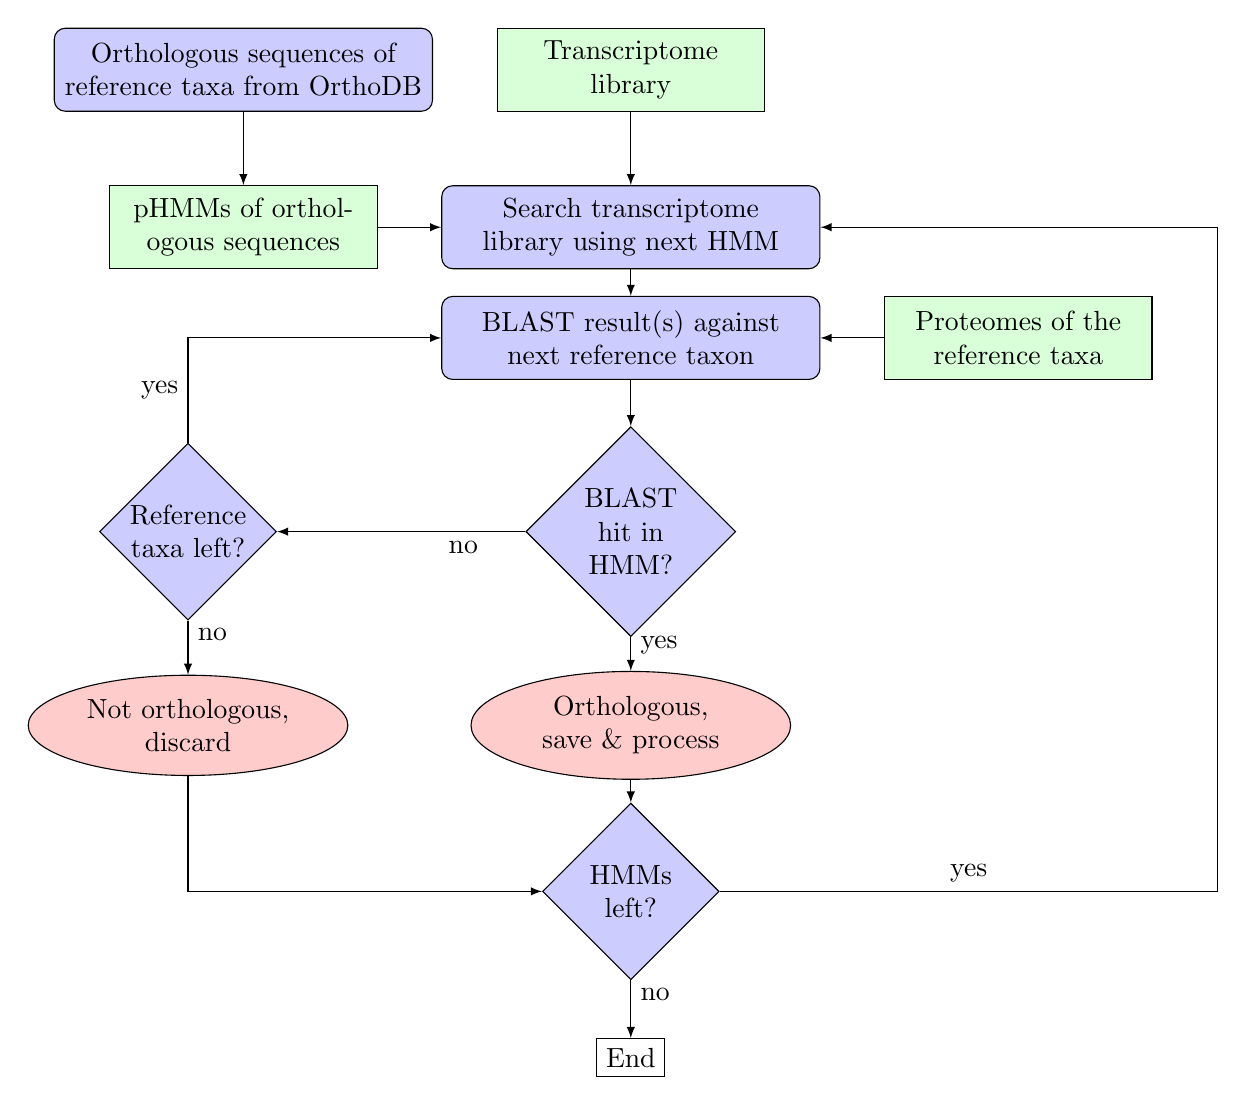
\begin{tikzpicture}[node distance = 2cm, auto]
	% nodes
	\node[rect] (transcriptome) {Transcriptome library};
	\node[block, below of = transcriptome] (hmmsearch) {Search transcriptome library using next HMM};
	\node[rect, left of = hmmsearch, node distance = 14em] (orthologs) {pHMMs of orthologous sequences};
	\node[block, above of = orthologs] (orthodb) {Orthologous sequences of reference taxa from OrthoDB};
	\node[block, below of = hmmsearch, node distance = 4em] (hmmhits) {BLAST result(s) against next reference taxon};
	\node[decision, below of = hmmhits, node distance = 7em] (blast) {BLAST hit in HMM?};
	\node[rect, right of = hmmhits, node distance = 14em] (proteomes) {Proteomes of the reference taxa};
	\node[cloud, below of = blast, node distance=7em] (orthologous) {Orthologous, save \& process};
	\node[decision, below of = orthologous, node distance = 6em] (hmmsleft) {HMMs left?};
	\node[decision, left of = blast, node distance = 16em] (reftaxaleft) {Reference taxa left?};
	\node[cloud, below of = reftaxaleft, node distance = 7em] (notorthologous) {Not orthologous, discard};
	\node[draw, below of = hmmsleft, node distance = 6em] (end) {End};

	% lines
	\path[line](transcriptome) -- (hmmsearch);
	\path[line](orthodb) -- (orthologs);
	\path[line](orthologs) -- (hmmsearch);
	\path[line](hmmsearch) -- (hmmhits);
	\path[line](proteomes) -- (hmmhits);
	\path[line](hmmhits) -- (blast);
	\path[line](blast) -- node[near start]{no} (reftaxaleft);
	\path[line](blast) -- node[near start]{yes} (orthologous);
	\path[line](orthologous) -- (hmmsleft);
	\path[line](hmmsleft) -| node[near start]{yes} ([xshift = 18.0em]hmmsleft.east) |- (hmmsearch);
	\path[line](reftaxaleft) |- node[near start]{yes} (hmmhits);
	\path[line](reftaxaleft) -- node[near start]{no} (notorthologous);
	\path[line](notorthologous) |- (hmmsleft);
	\path[line](hmmsleft) -- node[near start] {no} (end);
\end{tikzpicture}
